\documentclass[12pt,twoside]{article}
\usepackage{minted}
\usepackage[dvipsnames]{xcolor}
\usepackage{tikz,graphicx,amsmath,amsfonts,amscd,amssymb,bm,cite,epsfig,epsf,url}
\usepackage[hang,flushmargin]{footmisc}
\usepackage[colorlinks=true,urlcolor=blue,citecolor=blue]{hyperref}
\usepackage{amsthm,multirow,wasysym,appendix}
\usepackage{array,subcaption} 
% \usepackage[small,bf]{caption}
\usepackage{bbm}
\usepackage{pgfplots}
\usetikzlibrary{spy}
\usepgfplotslibrary{external}
\usepgfplotslibrary{fillbetween}
\usetikzlibrary{arrows,automata}
\usepackage{thmtools}
\usepackage{blkarray} 
\usepackage{textcomp}
\usepackage[left=0.8in,right=1.0in,top=1.0in,bottom=1.0in]{geometry}
\usepackage{pifont}
\usepackage{tikz-qtree}

%% Probability operators and functions
%
% \def \P{\mathrm{P}}
\def \P{\mathrm{P}}
\def \E{\mathrm{E}}
\def \Var{\mathrm{Var}}
\let\var\Var
\def \Cov {\mathrm{Cov}} \let\cov\Cov
\def \MSE {\mathrm{MSE}} \let\mse\MSE
\def \sgn {\mathrm{sgn}}
\def \R {\mathbb{R}}
\def \C {\mathbb{C}}
\def \N {\mathbb{N}}
\def \Z {\mathbb{Z}}
\def \cV {\mathcal{V}}
\def \cS {\mathcal{S}}

\newcommand{\RR}{\ensuremath{\mathbb{R}}}

\DeclareMathOperator*{\argmin}{arg\,min}
\DeclareMathOperator*{\argmax}{arg\,max}
\newcommand{\red}[1]{\textcolor{red}{#1}}
\newcommand{\blue}[1]{\textcolor{blue}{#1}}
\newcommand{\green}[1]{\textcolor{ForestGreen}{ #1}}
\newcommand{\fuchsia}[1]{\textcolor{RoyalPurple}{ #1}}



%
%% Probability distributions
%
%\def \Bern    {\mathrm{Bern}}
%\def \Binom   {\mathrm{Binom}}
%\def \Exp     {\mathrm{Exp}}
%\def \Geom    {\mathrm{Geom}}
% \def \Norm    {\mathcal{N}}
%\def \Poisson {\mathrm{Poisson}}
%\def \Unif    {\mathrm {U}}
%
\DeclareMathOperator{\Norm}{\mathcal{N}}

\newcommand{\bdb}[1]{\textcolor{red}{#1}}

\newcommand{\ml}[1]{\mathcal{ #1 } }
\newcommand{\wh}[1]{\widehat{ #1 } }
\newcommand{\wt}[1]{\widetilde{ #1 } }
\newcommand{\conj}[1]{\overline{ #1 } }
\newcommand{\rnd}[1]{\tilde{ #1 } }
\newcommand{\rv}[1]{ \rnd{ #1}  }
\newcommand{\rM}{\rnd{ m}  }
\newcommand{\rx}{\rnd{ x}  }
\newcommand{\ry}{\rnd{ y}  }
\newcommand{\rz}{\rnd{ z}  }
\newcommand{\ra}{\rnd{ a}  }
\newcommand{\rb}{\rnd{ b}  }
\newcommand{\rt}{\rnd{ t}  }
\newcommand{\rs}{\rnd{ s}  }


\newcommand{\rpc}{\widetilde{ pc}  }
\newcommand{\rndvec}[1]{\vec{\rnd{#1}}}

\def \cnd {\, | \,}
\def \Id { I }
\def \J {\mathbf{1}\mathbf{1}^T}

\newcommand{\op}[1]{\operatorname{#1}}
\newcommand{\setdef}[2]{ := \keys{ #1 \; | \; #2 } }
\newcommand{\set}[2]{ \keys{ #1 \; | \; #2 } }
\newcommand{\sign}[1]{\op{sign}\left( #1 \right) }
\newcommand{\trace}[1]{\op{tr}\left( #1 \right) }
\newcommand{\tr}[1]{\op{tr}\left( #1 \right) }
\newcommand{\inv}[1]{\left( #1 \right)^{-1} }
\newcommand{\abs}[1]{\left| #1 \right|}
\newcommand{\sabs}[1]{| #1 |}
\newcommand{\keys}[1]{\left\{ #1 \right\}}
\newcommand{\sqbr}[1]{\left[ #1 \right]}
\newcommand{\sbrac}[1]{ ( #1 ) }
\newcommand{\brac}[1]{\left( #1 \right) }
\newcommand{\bbrac}[1]{\big( #1 \big) }
\newcommand{\Bbrac}[1]{\Big( #1 \Big)}
\newcommand{\BBbrac}[1]{\BIG( #1 \Big)}
\newcommand{\MAT}[1]{\begin{bmatrix} #1 \end{bmatrix}}
\newcommand{\sMAT}[1]{\left(\begin{smallmatrix} #1 \end{smallmatrix}\right)}
\newcommand{\sMATn}[1]{\begin{smallmatrix} #1 \end{smallmatrix}}
\newcommand{\PROD}[2]{\left \langle #1, #2\right \rangle}
\newcommand{\PRODs}[2]{\langle #1, #2 \rangle}
\newcommand{\der}[2]{\frac{\text{d}#2}{\text{d}#1}}
\newcommand{\pder}[2]{\frac{\partial#2}{\partial#1}}
\newcommand{\derTwo}[2]{\frac{\text{d}^2#2}{\text{d}#1^2}}
\newcommand{\ceil}[1]{\lceil #1 \rceil}
\newcommand{\Imag}[1]{\op{Im}\brac{ #1 }}
\newcommand{\Real}[1]{\op{Re}\brac{ #1 }}
\newcommand{\norm}[1]{\left|\left| #1 \right|\right| }
\newcommand{\norms}[1]{ \| #1 \|  }
\newcommand{\normProd}[1]{\left|\left| #1 \right|\right| _{\PROD{\cdot}{\cdot}} }
\newcommand{\normTwo}[1]{\left|\left| #1 \right|\right| _{2} }
\newcommand{\normTwos}[1]{ \| #1  \| _{2} }
\newcommand{\normZero}[1]{\left|\left| #1 \right|\right| _{0} }
\newcommand{\normTV}[1]{\left|\left| #1 \right|\right|  _{ \op{TV}  } }% _{\op{c} \ell_1} }
\newcommand{\normOne}[1]{\left|\left| #1 \right|\right| _{1} }
\newcommand{\normOnes}[1]{\| #1 \| _{1} }
\newcommand{\normOneTwo}[1]{\left|\left| #1 \right|\right| _{1,2} }
\newcommand{\normF}[1]{\left|\left| #1 \right|\right| _{\op{F}} }
\newcommand{\normLTwo}[1]{\left|\left| #1 \right|\right| _{\ml{L}_2} }
\newcommand{\normNuc}[1]{\left|\left| #1 \right|\right| _{\ast} }
\newcommand{\normOp}[1]{\left|\left| #1 \right|\right|  }
\newcommand{\normInf}[1]{\left|\left| #1 \right|\right| _{\infty}  }
\newcommand{\proj}[1]{\mathcal{P}_{#1} \, }
\newcommand{\diff}[1]{ \, \text{d}#1 }
\newcommand{\vc}[1]{\boldsymbol{\vec{#1}}}
\newcommand{\rc}[1]{\boldsymbol{#1}}
\newcommand{\vx}{\vec{x}}
\newcommand{\vy}{\vec{y}}
\newcommand{\vz}{\vec{z}}
\newcommand{\vu}{\vec{u}}
\newcommand{\vv}{\vec{v}}
\newcommand{\vb}{\vec{\beta}}
\newcommand{\va}{\vec{\alpha}}
\newcommand{\vaa}{\vec{a}}
\newcommand{\vbb}{\vec{b}}
\newcommand{\vg}{\vec{g}}
\newcommand{\vw}{\vec{w}}
\newcommand{\vh}{\vec{h}}
\newcommand{\vbeta}{\vec{\beta}}
\newcommand{\valpha}{\vec{\alpha}}
\newcommand{\vgamma}{\vec{\gamma}}
\newcommand{\veta}{\vec{\eta}}
\newcommand{\vnu}{\vec{\nu}}
\newcommand{\rw}{\rnd{w}}
\newcommand{\rvnu}{\vc{\nu}}
\newcommand{\rvv}{\rndvec{v}}
\newcommand{\rvw}{\rndvec{w}}
\newcommand{\rvx}{\rndvec{x}}
\newcommand{\rvy}{\rndvec{y}}
\newcommand{\rvz}{\rndvec{z}}
\newcommand{\rvX}{\rndvec{X}}


\newtheorem{theorem}{Theorem}[section]
% \declaretheorem[style=plain,qed=$\square$]{theorem}
\newtheorem{corollary}[theorem]{Corollary}
\newtheorem{definition}[theorem]{Definition}
\newtheorem{lemma}[theorem]{Lemma}
\newtheorem{remark}[theorem]{Remark}
\newtheorem{algorithm}[theorem]{Algorithm}

% \theoremstyle{definition}
%\newtheorem{example}[proof]{Example}
\declaretheorem[style=definition,qed=$\triangle$,sibling=definition]{example}
\declaretheorem[style=definition,qed=$\bigcirc$,sibling=definition]{application}

%
%% Typographic tweaks and miscellaneous
%\newcommand{\sfrac}[2]{\mbox{\small$\displaystyle\frac{#1}{#2}$}}
%\newcommand{\suchthat}{\kern0.1em{:}\kern0.3em}
%\newcommand{\qqquad}{\kern3em}
%\newcommand{\cond}{\,|\,}
%\def\Matlab{\textsc{Matlab}}
%\newcommand{\displayskip}[1]{\abovedisplayskip #1\belowdisplayskip #1}
%\newcommand{\term}[1]{\emph{#1}}
%\renewcommand{\implies}{\;\Rightarrow\;}



\begin{document}

\begin{center}
{\large{\textbf{Homework 9}} } \vspace{0.2cm}\\
Due Apr 9 at 11 pm
\\
\end{center}
Unless stated otherwise, justify any answers you give.
You can work in groups, but each
student must write their own solution based on their own
understanding of the problem.

When uploading your homework to Gradescope you will have to
select the relevant pages for each question.  Please submit each
problem on a separate page (i.e., 1a and~1b can be on the same page but 1
and 2 must be on different pages).  We understand that this may be
cumbersome but this is the best way for the grading team to grade your
homework assignments and provide feedback in a timely manner.  Failure
to adhere to these guidelines may result in a loss of points.
Note that it may take some time to
select the pages for your submission.  Please plan accordingly.  We
suggest uploading your assignment at least 30 minutes before the deadline
so you will have ample time to select the correct pages for your
submission.  If you are using \LaTeX, consider using the minted or
listings packages for typesetting code.  
\\

\begin{enumerate}

\item (Normalization) In this problem we study the effect of normalizing by the standard deviation before performing principal component analysis. Let $\rx$ be a zero-mean $3$-dimensional random vector with covariance matrix 
\begin{align}
\Sigma_{\rx} := \MAT{ 100 & 25 & 0 \\ 25 & 400 & 0 \\ 0 & 0 & 0.16 }.
\end{align}
We define the normalized vector $\ry$ as
\begin{align}
\ry[i] := \frac{ \rx[i]}{ \sqrt{\var (\rx[i])}} \quad 1 \leq i \leq 3.
\end{align}
\begin{enumerate}
\item Compute the covariance matrix of $\ry$.  
\begin{itemize}
  \color{blue}
  \item observe that the random vector $\Tilde{y}\in \mathbb{R}^{3}$ can be written as $\Tilde{y}=v*\Tilde{x}$ that is as the element-wise 
  product of the original random vector $\Tilde{x}\in \mathbb{R}^{3}$ and the vector $v=\begin{pmatrix}
    \frac{1}{\sqrt{\Tilde{x}[1]}}\\\frac{1}{\sqrt{\Tilde{x}[2]}}\\\frac{1}{\sqrt{\Tilde{x}[3]}}
  \end{pmatrix}$
  \item then we can consider each of the elements of the new covariance matrix $\Sigma_{\Tilde{y}}$
  \item note that $\Sigma_{\Tilde{y}}[i,j]=cov(\Tilde{y}[i],\Tilde{y}[j])=cov(\frac{1}{\sqrt{\Tilde{x}[i]}}\Tilde{x}[i],\frac{1}{\sqrt{\Tilde{x}[j]}}\Tilde{x}[j])=
  E[\frac{1}{\sqrt{\Tilde{x}[i]}}\Tilde{x}[i]*\frac{1}{\sqrt{\Tilde{x}[j]}}\Tilde{x}[j]]-E[\frac{1}{\sqrt{\Tilde{x}[i]}}]\Tilde{x}[i]E[\frac{1}{\sqrt{\Tilde{x}[j]}}\Tilde{x}[j]]=\frac{1}{\sqrt{\Tilde{x}[i]}}\frac{1}{\sqrt{\Tilde{x}[j]}}(E[\Tilde{x}[i]\Tilde{x}[j]]-E[\Tilde{x}[i]]E[\Tilde{x}[j]])$
$ \\=\frac{1}{\sqrt{\Tilde{x}[i]}}\frac{1}{\sqrt{\Tilde{x}[j]}}cov(\Tilde{x}[i], \Tilde{x}[j])$
\item computing this out we get $\Sigma_{\Tilde{y}}=\begin{pmatrix}
  1 & \frac{1}{4} & 0\\\frac{1}{4} & 1 & 0 \\ 0 & 0 & 1
\end{pmatrix}$
\end{itemize}

\item Is the directional variance of $\ry$ equal to one in every direction?  
\begin{itemize}
  \color{blue}
  % \item consider the vector 
  % \item consider an arbitrary deterministic vector $a'\in \mathbb{R}^{3}$
  % \item we can define a new vector based on $a=\frac{a}{||a'||_{2}}$ as a normalized version of a'
  % \item 
  % \item the directional variance of $\Tilde{y}$ in the direction of a is the variance of 
  % the projection of $\Tilde{y}$ onto that dimension that is $P_{a}(\Tilde{y})=\frac{a^{t}\Tilde{y}}{||a||_{2}}=a^{t}\Tilde{y}$
  % \item we can see $var(a^{t}\Tilde{y})=a^{t}\Sigma_{\Tilde{y}}a=$
  \item this is false 
  \item consider the vector $a=\begin{pmatrix}
    \frac{1}{\sqrt{3}} \\ \frac{1}{\sqrt{3}}  \\ \frac{1}{\sqrt{3}}
  \end{pmatrix}$ 
  \item we know the variance of $\Tilde{y}$ in the direction of a is given by the variance of the projection of $\Tilde{y}$
  onto a 
  \item the projection $P_{a}(\Tilde{y})=\frac{a^t\Tilde{y}}{||a||}=a^{t}\Tilde{y}$
  \item then we know $var(P_{a}(\Tilde{y}))=var(a^t\Tilde{y})=a^{t}\Sigma_{\Tilde{y}}a$
  \item then computing this out we can see $var(P_{a}(\Tilde{y}))= 1.08333333\neq 1$
\end{itemize}


\item We decide to reduce the dimensionality of $\rx$ and $\ry$ to two dimensions using PCA. Report what directions are selected for each of the random vectors. (Feel free to use a computer for your calculations, but explain what you are doing.)  
\begin{itemize}
  \color{blue}
  \item given we would like to reduce the dimensionality of our random vector $\Tilde{x}\in \mathbb{R}^{d}$ to $k\leq d$
  \item our steps are first to find the covariance $\Sigma_{\Tilde{x}}$
  \item then we compute an eigendecomposition of $\Sigma_{\Tilde{x}}$ and take it's top k eigenvectors $u_1\dots u_k$, as by the spectral theorem these are the directions of maximal variance for the random vector $\Tilde{y}$
  \item then we project $\Tilde{y}$ back onto those directions to get the k principal components of $\Tilde{y}$ $p_1...p_k=P_{u_1}(\Tilde{x})\dots P_{u_k}(\Tilde{x})=\frac{u_1^{t}\Tilde{x}}{||u_1||_2}\dots \frac{u_k^{t}\Tilde{x}}{||u_k||_2}=u_1^{t}\Tilde{x}\dots u_k^{t}\Tilde{x}$
  \item we can apply this methodology to our problem by looking at the random vector $\Tilde{y}$ with k=2
  \item we can compute the eigenvalues of our covariance matrix as $\begin{pmatrix}
    1.125\\ 0.875\\ 1.  
  \end{pmatrix} $
  \item  and see that $1.125, 1$ are our largest two eigenvalues
  \item then we can find the principal directions of our data as there associated eigenvectors
  which are $\lambda_1=1.125, u_1=\begin{pmatrix}
    0.70710678 \\0.70710678 \\0
  \end{pmatrix}$ and $\lambda_2=1, u_2=\begin{pmatrix}
    0 \\0 \\1
  \end{pmatrix}$
\end{itemize}
\item Explain which of the two options for dimensionality reduction to 2D would make more sense in each of the following situations and why that is the case: (1) The entries of $\rx$ represent the weight (in kilograms), heart rate (in beats per minute), and height (in meters) of a set of hospital patients. (2) The entries of $\rx$ represent the length, width and height (all in centimeters) of a set of cars.  

\begin{itemize}
  \color{blue}
  \item i think dimensionality reduction makes more sense in case a. 
  \item in case a we are dealing with health data. each of our quantities is potentially related
  that is for example someones weight and height could have notable information about there 
  heart rate. Further, in case a we are trying to understand health outcomes so reducing this 
  data to principal directions that may be a mixture of features could tell us something 
  integrable about health care outcomes 
  \item option b on the other hand is dealing with the dimensions of objects (in this case cars)
  and there may not be a strong corelation between the features. For instance 
  knowing that a car is long may not tell you anything about its height or width
  for instance both a traditional limo and jeep limo are abnormally long, but they have 
  very different heights and widths. This further implies that in the case of objects taking
  principal directions that may be a combination of multiple features may not be useable.
  Further, the data in this set already exists in a
  form that can be understood in 3 dimensions so dimensionality reduction is kind of pointless. 

\end{itemize}


\end{enumerate} 

\item (Faces) The following questions refer to the code in the folder {\tt faces }
  The Olivetti faces dataset used in  {\tt faces }  contains images of faces of people associated with a unique numeric id to identify the person.
 
\begin{enumerate}
\item  Complete the \verb|compute_nearest_neighbors()| function in \verb|nearest_neighbors.py| that finds the image in the training data that is closest to a given test image.  Include the generated images in your submitted homework.
\begin{itemize}
\item \inputminted[firstline=39, lastline=42, breaklines=True]{python}{hw9.py}


\end{itemize}


\vspace{0.5cm}Create a new file in which
you must write code to complete the following tasks:

\item Generate a plot of $k$ vs.~$\sigma^2_k$, where $\sigma^2_k$ is
the variance of the $k$th principal component of the data (e.g., $\sigma^2_1$
is the largest variance). 
Include the plot in your submitted homework document. You can limit the x axis to a reasonable number.
\begin{itemize}
\item \inputminted[firstline=52, lastline=64, breaklines=True]{python}{hw9.py}
\item 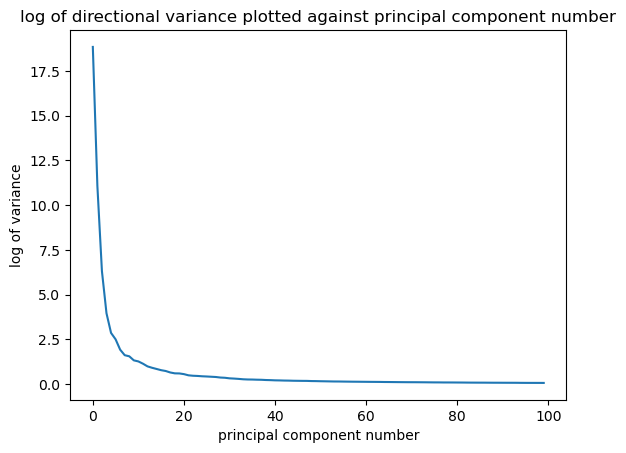
\includegraphics[width=10cm]{homework/homework_9/images/hw9_1.png}
\end{itemize}


\item  Plot (using  \verb|plot_image_grid()| in
\verb|plot_tools.py| ) the vectors
corresponding to the top 10 principal directions of the data.

reasonable number.
\begin{itemize}
\item \inputminted[firstline=67, lastline=83, breaklines=True]{python}{hw9.py}
\item 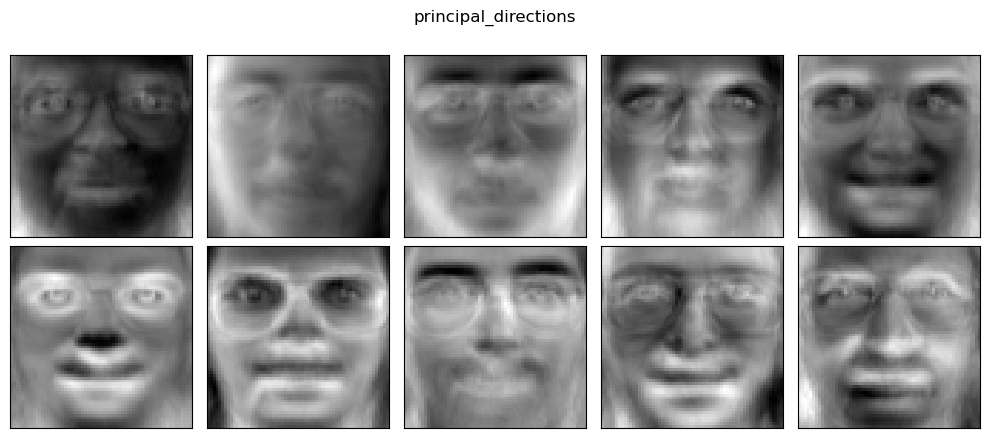
\includegraphics[width=10cm]{homework/homework_9/images/hw9_2.png}
\end{itemize}

Your principal direction vectors should be in $\mathbb{R}^{4096}$ (they represent images).
Include the plot in your submitted homework document.
\item Use the variance of principal directions plot to determine a 
relatively small number $k$ of principal components
that explains the training data reasonably well.
Project the training data 
and the test data onto the
first $k$ principal components, and run nearest neighbors for
each test image in this lower dimensional space.  Include your
choice for $k$, and the plots
of your nearest neighbor results in your submitted homework
document.  You should use the code from
 \verb|nearest_neighbors.py| to generate your image plots.
reasonable number.
\begin{itemize}
\item \inputminted[firstline=92, lastline=124, breaklines=True]{python}{hw9.py}
\item 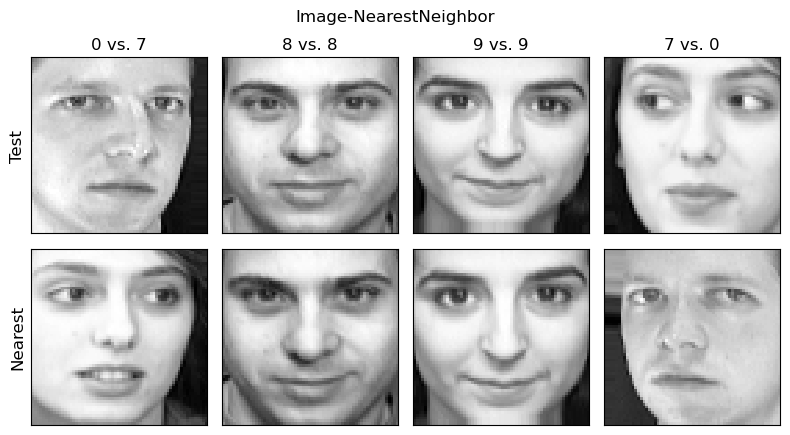
\includegraphics[width=10cm]{homework/homework_9/images/hw9_3.png}
\end{itemize}
 
\item Give a reason why applying 
nearest-neighbor approach after performing dimensionality reduction could potentially produce better results.
\begin{itemize}
    \item we are filtering out dimensions that may be noise (that is may relate to things like the position the picture was taken in) and only focusing on features that are relevant to the face shape (ideally). then we are able to compare distance, a way that is more directly relvent to the faces.
\end{itemize}


% \item Use \verb|sklearn.cluster.KMeans| to perform KMeans on the entire dataset (both train and test set) with $k=40$. Use \verb|plot_image_grid()| to create a picture of all the $k$ cluster centers. 
\end{enumerate}

  Some notes to keep in mind:
  \begin{enumerate}
  \item The function {\tt np.linalg.eig} might return complex eigenvectors.
  \item The data points in the training and test data are given as
    rows.
    \item Include all new code (or functions) you have filled in your final PDF.
 \end{enumerate}

 \end{enumerate}
 
\end{document}
